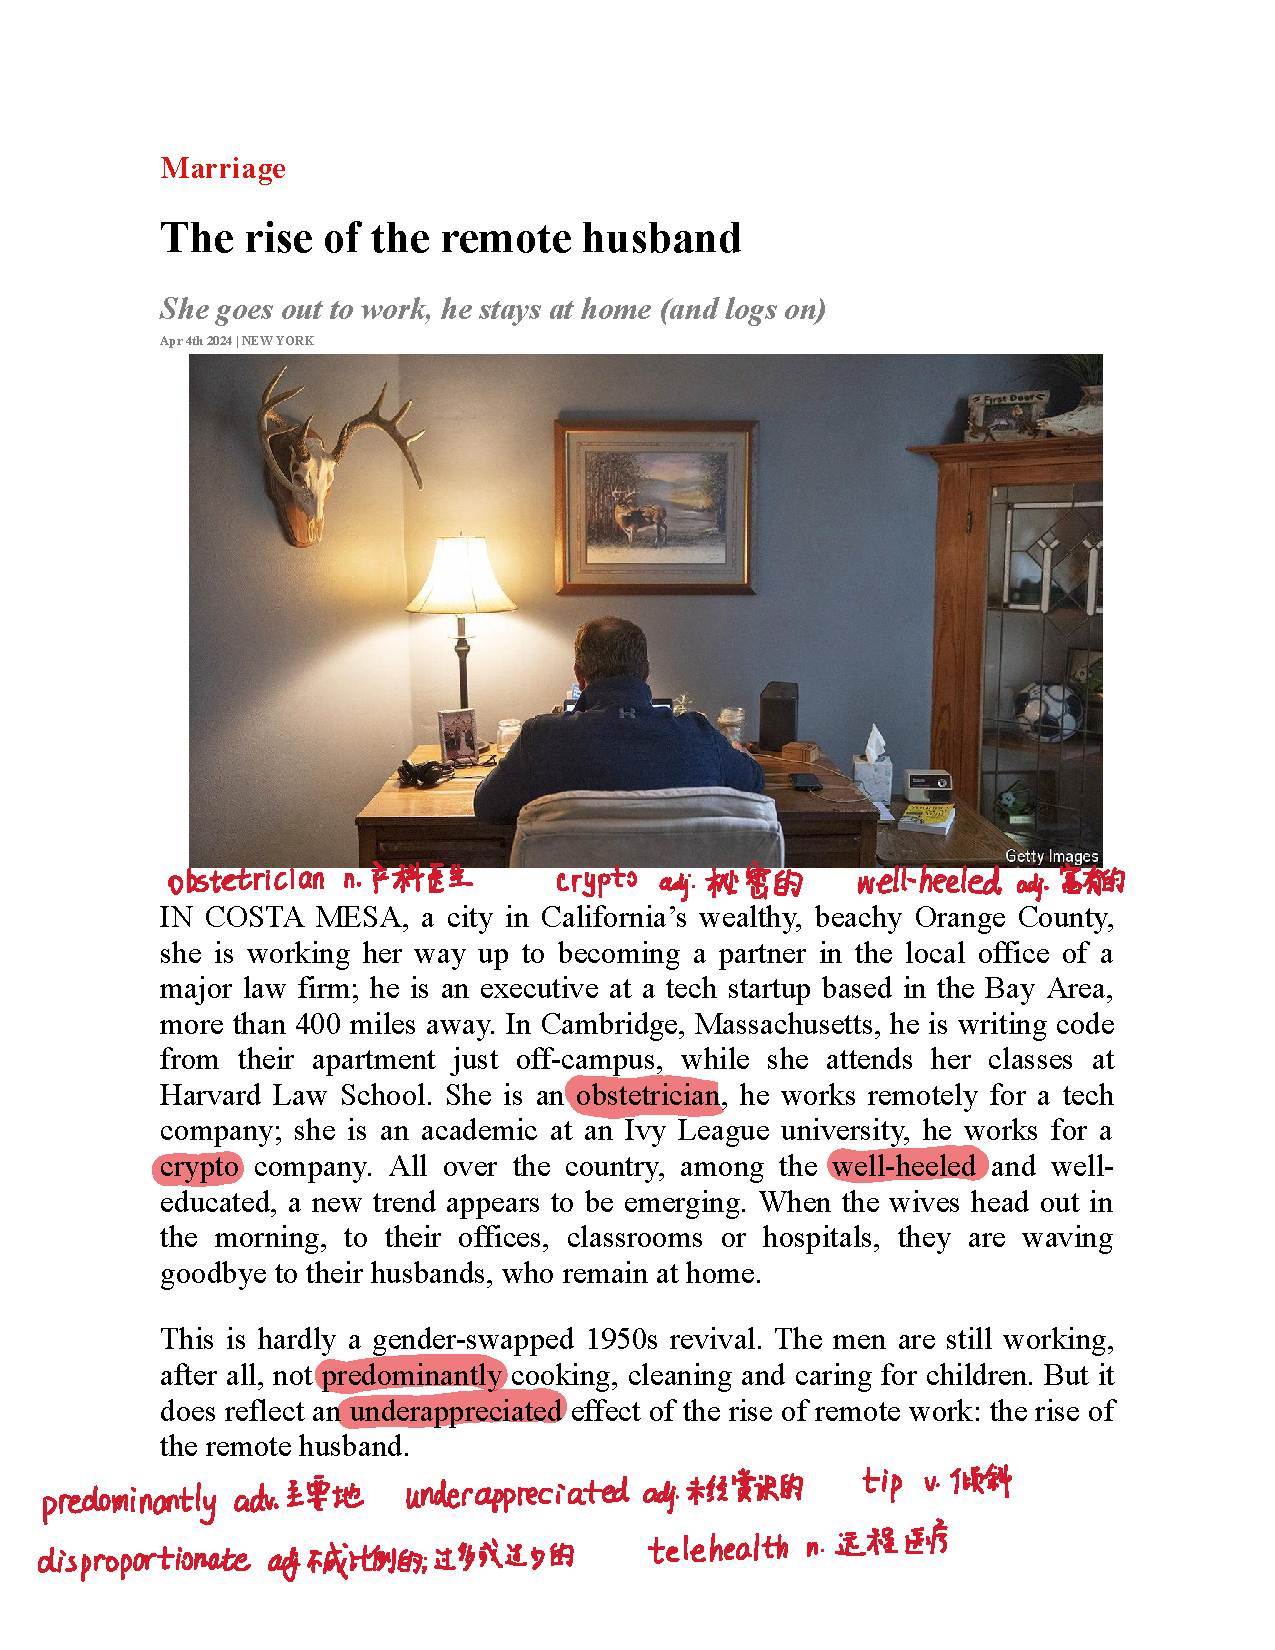
\includepdf[pages={1-3}]{第七周外刊.pdf}
\begin{itemize}
    \item [1.]Ivy League 常春藤名校联盟
    \begin{multicols}{2}
        \begin{itemize}
            \item [a.]哈佛Harvard
            \item [b.]宾大University of Pennsylvania
            \item [c.]耶鲁Yale University
            \item [d.]普林斯顿Princeton University
            \item [e.]哥大Columbia University
            \item [f.]布朗Brown University
            \item [g.]康奈尔Cornell University
            \item [h.]达特茅斯Dartmouth College
        \end{itemize}
    \end{multicols}
    
    \item [2.]crypto company 加密公司
    \item [3.]underappreciated adj. 尚未被重视的,低估的


    e.g.\qquad Yet, \textbf{an underappreciated effect of} increased 
    social media usage \textbf{is its impact on }
    interpersonal skills. \textbf{While much focus is 
    placed on the benefits of }instant communication, 
    \textbf{such as }increased information sharing and 
    connectivity, \textbf{the consequences of }
    reduced face-to-face interactions on our 
    ability to effectively communicate and 
    empathize with others \textbf{are often overlooked. 
    This decline in }social skills can lead to 
    a deeper sense of isolation and misunderstanding 
    in society, \textbf{despite }the virtual connectivity.

    (...的坏处常常被低估,它的可能后果是...)
    \item [4.]swap v. 互换、交换
        
    swap A for B 把A换成B(可用于作文中措施段,用...替换...)


    congestion n. 交通堵塞


    e.g.\qquad ...(环保措施), which will encourage people to swap car travel 
    for cycling or walking to reduce traffic congestion 
    and air pollution.
    \item [5.]predominantly adv. 主要
    
    bolster v. 增强
    
    e.g.\qquad While traditional teaching methods and digital 
    tools play crucial roles in education, it is 
    predominantly online resources and software 
    applications that are shaping the way students 
    learn in many cultures. This trend towards 
    digitalization in education reflects broader societal 
    shifts towards technology reliance.
    \item [6.]disproportionate adj. 不匀称的,不均衡的
    
    a large proportion of ... ...的很大一部分

    a sense of proportion 有轻重缓急之分,分寸感

    out of proportion 比例失调,不匀称
    \item [7.]tip v. 倾斜,变化
    
    the scales are tipping as ... 随着...,情况正在反转

    e.g.1\qquad While artificial intelligence was once the domain 
    of science fiction, \textbf{the scales are tipping as }
    AI becomes an integral part of daily life, from 
    smart home devices to personalized healthcare solutions.

    underscore v. 强调
    
    traction n. 拉力

    gain traction 发展

    gig n. 临时工作

    e.g.2\qquad The conventional 9-to-5 office job has been the 
    standard for decades, symbolizing stability and 
    professional success. But \textbf{the scales are tipping, as }
    the gig economy and remote work \textbf{gain traction}. 
    This transformation underscores a reevaluation 
    of traditional work values, emphasizing 
    the importance of work-life balance, autonomy, 
    and \textbf{leveraging }technological advancements 
    to facilitate working from any location.

    the tip of the iceberg 冰山一角

    e.g.3\qquad These examples are just \textbf{the tip of the iceberg}, 
    but they demonstrate how helping 
    customers get more use of their materials can 
    transform value chains and operations.

    the tipping point 转折点

    e.g.4\qquad It looks like it---after all, 
    2012 was \textbf{the tipping point }when more than half 
    of Americans began owning smartphones.

    \item [8.]be tied to 被...束缚
    
    e.g.\qquad I dont't want to be tied to a steady job. 我不想被工作束缚
    $\rightarrow$我不想要一成不变的工作
    \item [9.]in aggregate 总的来说
    \item [10.]the short end of the stick 不利地位
    \item [11.]myopic adj. 目光短浅的
    
    e.g.\qquad (先说一个荒谬的观点)But the 
    view is myopic.(再接下文)
    \item [12.]disadvantage v. 对...不利
    
    e.g.1\qquad This may appear another development 
    where remote work \textbf{disadvantages }workers 
    by blurring the lines between personal and 
    professional life. \textbf{But that view is 
    myopic.} In reality, remote work offers 
    unprecedented flexibility, empowering individuals 
    to design work schedules that harmonize with 
    their personal lives and responsibilities.

    e.g.2\qquad This may sound like another example 
    of how technological advancements lead to greater 
    social isolation. \textbf{But that view is myopic}. 
    In reality, technology has the power to connect 
    people across geographical boundaries like 
    never before, fostering new communities and enabling 
    closer relationships despite physical distance.

    testament n. 证据,证明

    nuanced adj. 微妙的,细致入微的

    e.g.3\qquad This may sound like another testament
    to the belief that tecchnology can solve all our 
    problems. \textbf{But that view is myopic}. 
    In reality, while technological advancements 
    have undoubtedly improved many aspects of our 
    lives, they also pose new ethical dilemmas and 
    challenges. Issues such as privacy invasion, 
    data security, and the digital divide require a 
    nuanced understanding of ethics beyond mere 
    technical solutions.
\end{itemize}